\documentclass[12pt]{notes}

% Command for Questions
%\question{}

% Command for Notes
% \note{}

% Code to create a minipage where you can type in class notes. 
%%\begin{minipage}[l][2cm][c]{\textwidth}
\begin{comment}

\end{comment}
%%\end{minipage}

\usepackage{listings}

% In order for the minted code to run, we had to create a new compilation routine called pdflatex+shellEscape.
% This includes a --shell-escape command which should ONLY be used when pygmentized is required as it compromises security. 
% We also had to add pygmentize (a python package) to the system path (BEFORE miktex) and then restart the computer. 
\usepackage{minted}
\usemintedstyle{borland}
\lstset{language=SAS, 
  breaklines=true,  
  basicstyle=\ttfamily\bfseries,
  columns=fixed,
  keepspaces=true,
  identifierstyle=\color{blue}\ttfamily,
  keywordstyle=\color{cyan}\ttfamily,
  stringstyle=\color{purple}\ttfamily,
  commentstyle=\color{green}\ttfamily,
  } 
  
% \begin{minted}{sas}
% \end{minted}


% Begin Document
%==============================================================================
\begin{document}
% Include the Title of the Handout
\ntitle{2.2: Diagnostics and Remedial Measures}

% Include Numbered Sections
\section{Why Diagnostics}

Recall that the nice properties of the OLS coefficient estimates relied on the assumption that \[\epsilon \stackrel{iid}{\sim} N(0, \sigma^2).\]

\question{(Groups) What happens if the assumptions regarding residuals are not satisfied?}

\begin{minipage}[l][3cm][c]{\textwidth}
\begin{comment}
\note{The p-values associated with our model rely on proper assumptions regarding the test statistics' ``sampling distributions''.}

\note{If the residual assumptions are satisfied, then the sampling distributions are wrong and the p-values are worthless.}
\end{comment}
\end{minipage}

\subsection*{Model Assumptions in Linear Regression}
\begin{enumerate}
\item X and Y share a linear relationship
\begin{itemize}
\item X and Y can be related in a non-linear way, but OLS regression cannot be used in this case
\end{itemize}
\item model describes all observations 
\begin{itemize}
\item no outliers or influential points
\end{itemize}
\item additional predictor variables are unnecessary
\begin{itemize}
\item there is no additional information to ``extract'' from $\epsilon$
\end{itemize}
\item $\epsilon$'s follow a normal distribution
\begin{itemize}
\item Crucial for small sample sizes, not so critical for large ($> 500$) sample sizes due to central limit theorem. 
\end{itemize}
\item $\epsilon$'s have constant variance
\item $\epsilon$'s are independent (possibly related to item \#3)
\end{enumerate}

We check assumptions using \textbf{diagnostics} and fix violated assumptions using \textbf{remedial measures}. Violations are most apparent in the \textbf{error terms} ($\epsilon_1, \ldots, \epsilon_n$) so we focus on \textbf{residuals} ($e_1 \ldots e_n$). 

\nspace
There are both \textbf{graphical} and \textbf{numerical} checks of the assumptions regarding residuals, but the graphical assumptions are more informative. 

\begin{figure}[H]
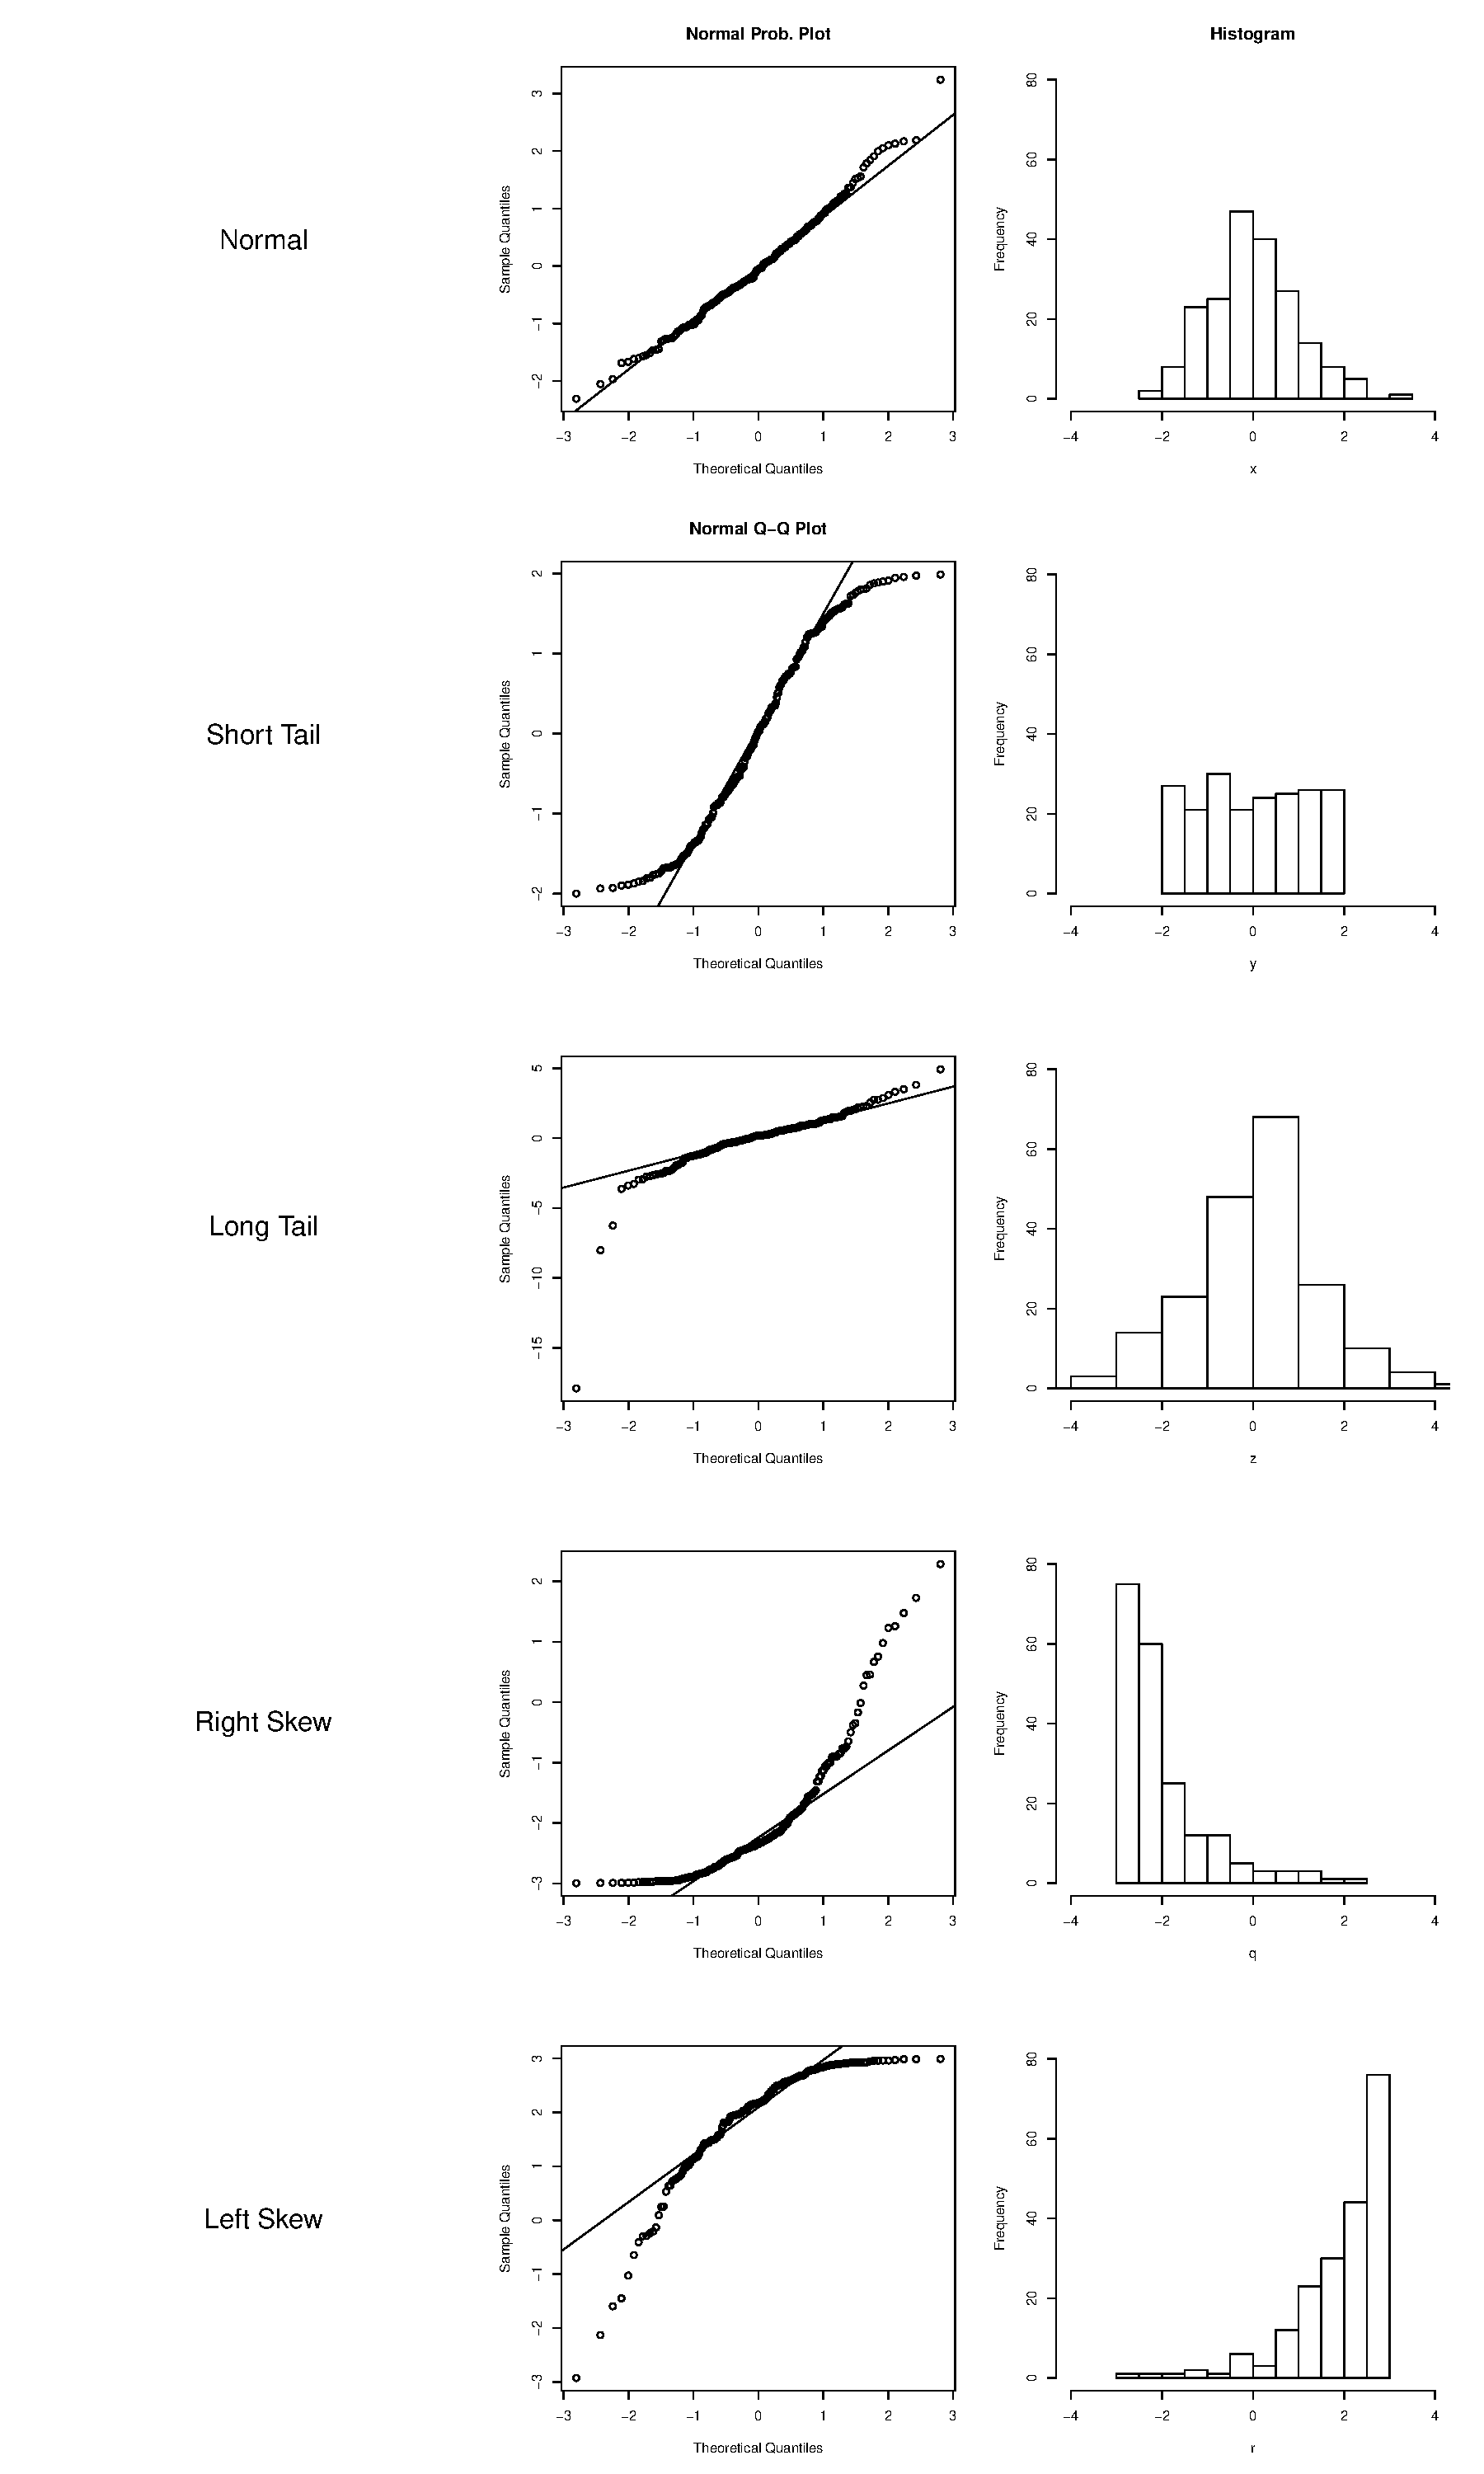
\includegraphics[width = 0.8\textwidth]{figures/module2/distTable.pdf}
\caption{Example scatterplot and histograms for different data distributions.}
\end{figure}

\section{Graphical Diagnostics}
\begin{itemize}
\item \textbf{Boxplot:} quick way to check for the symmetry of residuals. 
\item \textbf{Histogram:} Way to check the shape of a distribution. 
\begin{itemize}
\item SAS will overlay a normal curve on the histogram of residuals to help check for normality. 
\end{itemize}
\item \textbf{Normal Probability Plot:} a qq-plot where the quantiles of the data are compared to the expected quantiles under a normal distribution
\begin{itemize}
\item Expected values under normality have a mean of $0$ and a SD = $\sqrt{\text{MSE}}.$
\item See page 111 in textbook for method for details about how to approximate expected observations under normality.  
\item If data are approximately normal, the residuals in the Normal Probability Plot should closely follow a straight line. 
\end{itemize}
\item \textbf{Sequence Plot:} Line plot with residual values on the X axis and observation number on the X-axis. 
\begin{itemize}
\item Can ``connect'' the dots because there is only one Y value for every X value. 
\item Look for patterns in the residuals across time/observation number. 
\end{itemize}
\item \textbf{Residual Plot}
\begin{itemize}
\item Plot $e$ vs $X$ or $e$ vs $\hat{Y}$
\item Look for non-linearity and or non-constant variance in these scatterplots.  
\end{itemize}
\end{itemize}

\begin{figure}[H]
\centering
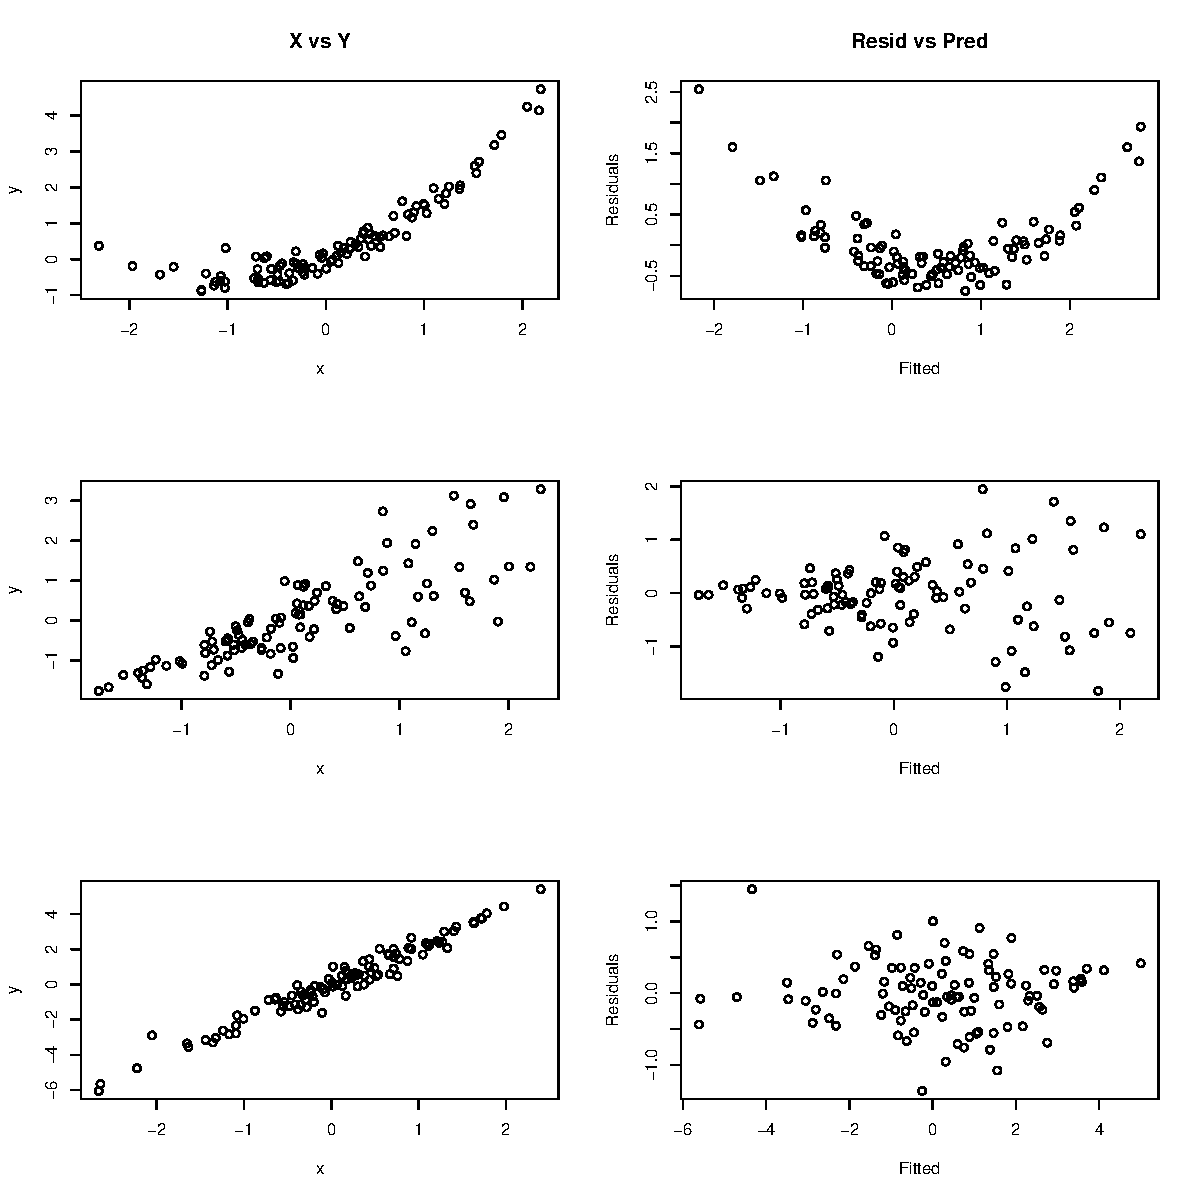
\includegraphics[width = 0.5\textwidth]{figures/module2/linPlots.pdf}
\caption{Plots showing 1) non-linearity, 2) non-constant variance, and 3) satisfied assumptions.}
\end{figure}

\section{Numerical Diagnostics}
Numerical diagnostics seek to determine if violations of model assumptions are statistically significant. 

\question{(Groups) Why would graphical checks of assumptions be preferred to numerical checks of significance.}

\begin{minipage}[l][3cm][c]{\textwidth}
\begin{comment}
\note{Violations of assumptions occur on a spectrum, numerical tests try to force a binary decision.}

\note{Numerical tests are good to verify potential violations that you suspect based on graphical checks.}
\end{comment}
\end{minipage}

\nspace
\subsection{Some Numerical Tests}
\begin{itemize}
\item Broth-Forsythe (BF) test of constant variance:

\begin{figure}[H]
\centering
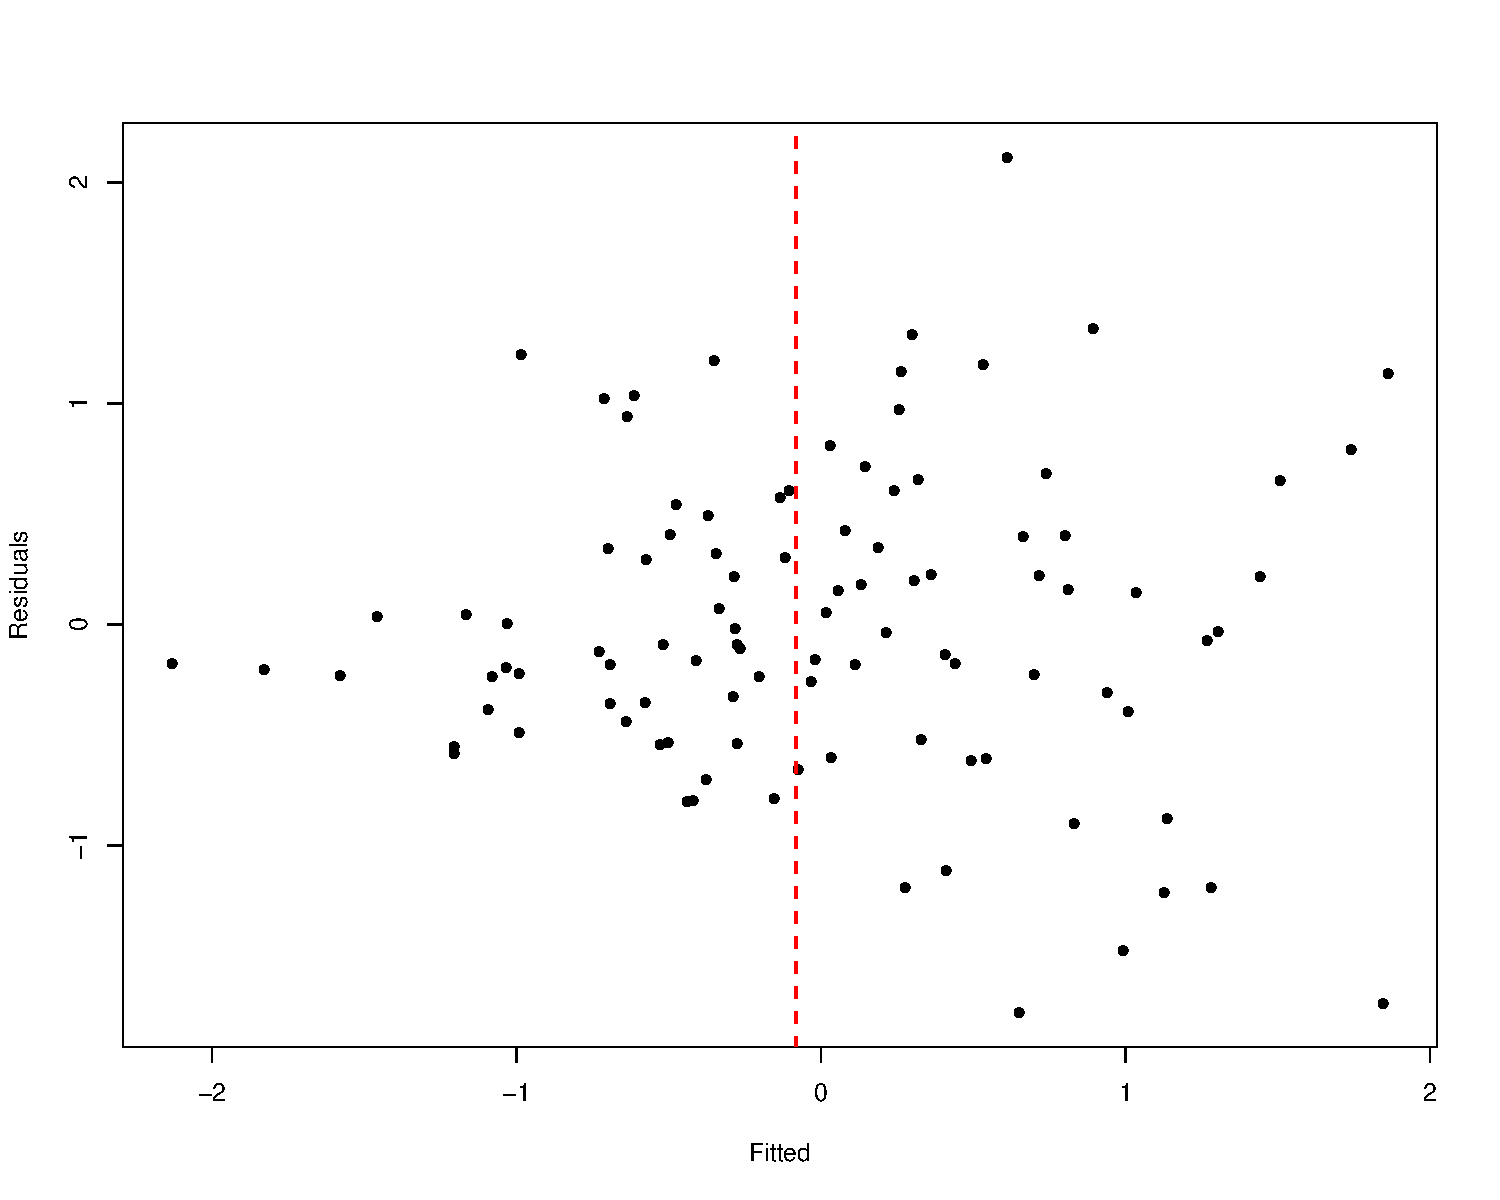
\includegraphics[width = 0.5\textwidth]{figures/module2/BFtest.pdf}
\end{figure}

\begin{itemize}
\item Split the data into two groups based on the median predicted value. 
\item Calculate the median absolute deviation (MAD) $d_i = |e_i - \tilde{e}|$, where $\tilde{e}$ is the median within each group (lower and upper). 
\item Conduct a two-sample t-test of d's to determine if the average of $d_i$'s within each group are significantly different.  
\item \textbf{Null Hypothesis: The variance of $\epsilon$ is constant.} (Estimated with residuals $e$).
\end{itemize}

\begin{minipage}[l][2cm][c]{\textwidth}
\begin{comment}
\note{Toluca Example: BF p-value is .2, which suggests there is not significant evidence of non-constant variance.}
\end{comment}
\end{minipage}

\item Correlation Test of Normality
\begin{itemize}
\item Calculate correlation between observed $e$'s and the ``normal-expected'' $e$'s ($e*$). Similar to expected residuals in qqplot. 
\item \textbf{Null hypothesis: $\epsilon$ follows a normal distribution.}
\item If the correlation isn't at least as big as the cirtical value for $\alpha=0.05$ in Table B.6 for a given sample size $n$, then reject $H_0$. 
\item \textbf{NOTE: The p-values provided in the SAS macro output mean \textit{nothing} for the correlation test of normality.} 
\end{itemize}

\begin{minipage}[l][2cm][c]{\textwidth}
\begin{comment}
\note{Toluca Example: Correlation of $0.992 > 0.96$, so there is not significant evidence of non-normality.}
\end{comment}
\end{minipage}

\item F-test for lack of fit (test of linearity between X and Y)
\begin{itemize}
\item See textbook 3.7 for details. 
\item Requires multiple observations at one or more X-levels. (Hard to do in observational studies or studies with multiple X-variables). 
\item Basically, the test compares the regression predictions to the empirical average of $Y$ at X-levels with multiple observations. 
\item \textbf{Null hypothesis: The regression function is linear.}   
\end{itemize}

\begin{minipage}[l][2cm][c]{\textwidth}
\begin{comment}
\note{Toluca Example: p-value $0.69 > .05$ suggests there is no significant evidence of non-linearity.}
\end{comment}
\end{minipage}
\end{itemize}

\begin{figure}[H]
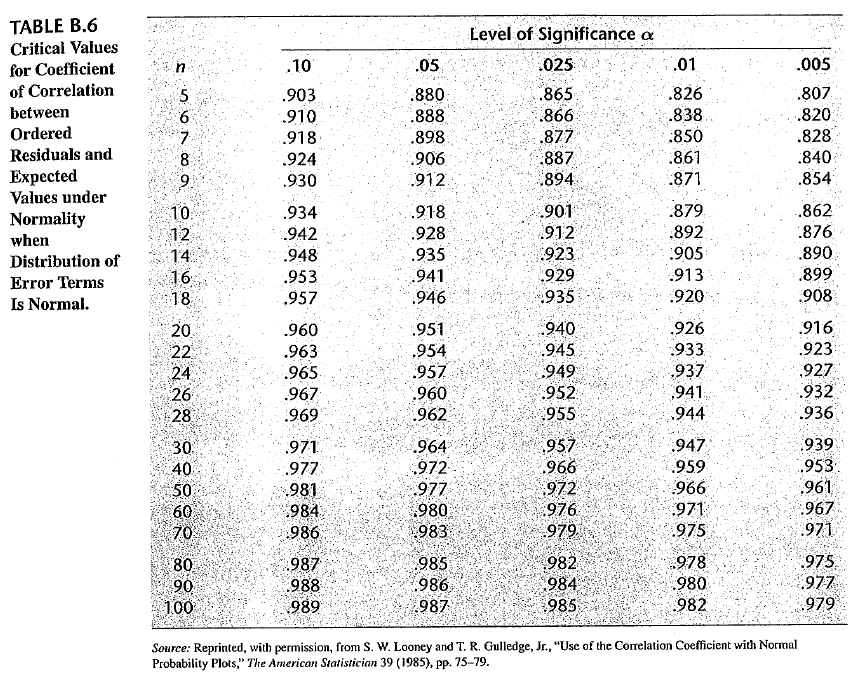
\includegraphics[width = \textwidth]{figures/module2/tableB6.png}
\end{figure}

\section{Remedial Measures}

If assumptions are violated, your options are:
\begin{itemize}
\item Give up (at least on linear regression). 
\item Alternatives to OLS like Regression Trees, Quantile Regression etc. (more later in the semester). 
\item Depending on the X vs Y relationship, try non-linear regression (more later in the semester). 
\item \textit{For non-normality and heteroskedasticity:} Variable Transformations on $X$ or $Y$ (not $e$). 
\begin{itemize}
\item Sometimes, a combination of transformations on both $X$ and $Y$ variables is needed. 
\item NOTE: Removing ``outlier'' points from a model should be seen as a measure of last resort. 
\end{itemize}
\end{itemize}

\subsection*{Box-Cox Approach}
% Box-Cox should not become your horoscope. 
Great starting point to determine candidate transformations, but no ``magical'' solution. 

\begin{itemize}
\item Define new response variable 
\[Y' = 
\begin{cases} 
\text{sign}(\lambda)Y^\lambda & \lambda \ne 0 \\
\log(Y) & \lambda = 0
\end{cases}
\]
(Note that $\text{sign}(\lambda)$ preserves the original ordering of the response variable). 
\item Consider the theoretical model
\[Y_i^\lambda = \beta_0 + \beta_1X_i + \epsilon_i\]
\item Consider a set of candidate lambda values, use maximum liklihood estimation to determine the ``best value.''
\begin{itemize}
\item Maximum likelihood estimation: ``which value of $\lambda$ is the most likely, given the data that I have observed?
\end{itemize}
\item \textbf{When possible: pick an \textit{interpretable} transformation that is close to the transformation recommended by SAS.}

\begin{minipage}[l][1cm][c]{\textwidth}
\begin{comment}
\note{Toluca Example: Ex: if $\lambda = .009$ is recommended, probably go with $\lambda = 0 \rightarrow \log(\lambda)$}
\end{comment}
\end{minipage}

\end{itemize}

In SAS:
\begin{minted}{sas}
proc transreg data=plasma;
 model boxcox(<response variable> / lambda=<lower> to <upper> by <step size>) 
       = identity(<explanatory variable) ...;
run;
\end{minted}

\subsection*{Omitted Predictors}
Think of regression as a form of data mining: we want to extract as much \textit{information} as we can from our \textit{data}.

\nspace
If we failed to extract all the information from the data, this may show up as a trend in the plot the residuals (which SHOULD have a constant mean of 0). 

\nspace
We will discuss more about how to extract \textit{time} related information in data at the end of the semester. 

\nspace
If you apply multiple methods to fix violations assumptions, make sure to check that the final model actually fixed the violations of assumptions. 
















% End the Document
%==============================================================================
\end{document}